\documentclass[11pt]{article}
% This is Marcus's style file, for little research notes and so on.  I
% keep this in $HOME/texmf/tex/latex, because kpsewhich
% -var-value=TEXMFHOME tells me that ($HOME/texmf) is where latex
% looks, at least under Ubuntu 12.10

\renewcommand{\familydefault}{\sfdefault} % use sans serif fonts
\usepackage{graphicx}
\usepackage[usenames]{color} % so you can {\color{red} anything}, etc.
\usepackage[fleqn]{amsmath}
\usepackage{amsmath}
\usepackage{amssymb,amsfonts}
\setlength{\textwidth}{16cm}
\setlength{\textheight}{24cm}
\hoffset=-2cm
\voffset=-2cm
\raggedbottom
\setlength{\parindent}{0in}
\setlength{\parskip}{0.14in plus 0.07in minus 0.07in}

\setcounter{tocdepth}{2} % determines the depth to which tableofcontents goes

%--------------------------------
\newcommand{\Line}[0]{\rule{0cm}{0cm}\\\hrule\rule{0cm}{0cm}}
\newcommand{\independent}{\protect\mathpalette{\protect\independenT}{\perp}}
\def\independenT#1#2{\mathrel{\rlap{$#1#2$}\mkern2mu{#1#2}}}
\newcommand{\dependent}{\not\independent}
\newcommand{\data}{\mathcal{D}}
\newcommand{\scriptL}{\mathcal{L}}
\newcommand{\mat}[1]{\ensuremath{\mathbf{#1}}} % vectors/matrices, x,A,B etc.
\newcommand{\gmat}[1]{\mbox{\boldmath${#1}$}}  % vectors/matrices Greek symbols
\newcommand{\swrt}[2]{\frac{\partial #1}{\partial #2}} % partial derivative of single symbol
\newcommand{\bwrt}[1]{\frac{\partial}{\partial #1}} % partial derivative of something big
\newcommand{\bA}{\mat{A}}
\newcommand{\ba}{\mat{a}}
\newcommand{\bg}{\mat{g}}
\newcommand{\bh}{\mat{h}}
\newcommand{\bw}{\mat{w}}
\newcommand{\bv}{\mat{v}}
\newcommand{\bx}{\mat{x}}
\newcommand{\by}{\mat{y}}
\newcommand{\bz}{\mat{z}}
\newcommand{\bp}{\mat{p}}
\newcommand{\br}{\mat{r}}
\newcommand{\bs}{\mat{s}}
\newcommand{\bt}{\mat{t}}
\newcommand{\bu}{\mat{u}}
\newcommand{\bm}{\mat{m}}
\newcommand{\bn}{\mat{n}}
\newcommand{\bc}{\mat{c}}
\newcommand{\bC}{\mat{C}}
\newcommand{\bH}{\mat{H}}
\newcommand{\bM}{\mat{M}}
\newcommand{\bT}{\mat{T}}
\newcommand{\bW}{\mat{W}}
\newcommand{\bX}{\mat{X}}
\newcommand{\bY}{\mat{Y}}
\newcommand{\bZ}{\mat{Z}}
\newcommand{\balpha}{\boldsymbol\alpha}
\newcommand{\bSigma}{\boldsymbol\Sigma}
\newcommand{\btheta}{\boldsymbol\theta}
\newcommand{\wo}{\mat{\backslash}}
\newcommand{\bCinv}{\mat{C}^{-1}}
\newcommand{\bCinvPrime}{\mat{C^\prime}^{-1}}
\newcommand{\bkNN}{\mat{k}}
\newcommand{\T}{\ensuremath{\textit{T}}}
\newcommand{\Dir}{\ensuremath{\text{Dir}}}

\newcommand{\Bel}[0]{\text{Bel}}
\newcommand{\on}[0]{\text{on}}
\newcommand{\off}[0]{\text{off}}
\newcommand{\ith}[0]{\text{$i^\text{th}\;$}}
\newcommand{\jth}[0]{\text{$j^\text{th}\;$}}
\newcommand{\kth}[0]{\text{$k^\text{th}\;$}}
\newcommand{\wth}[0]{\text{$w^\text{th}\;$}}
\newcommand{\dth}[0]{\text{$d^\text{th}\;$}}
\newcommand{\nth}[0]{\text{$n^\text{th}\;$}}
\newcommand{\tth}[0]{\text{$t^\text{th}\;$}}

\newcommand{\half}[0]{\text{\tiny$\frac{1}{2}$}}
\newcommand{\onethird}[0]{\text{\tiny$\frac{1}{3}$}}
\newcommand{\twothirds}[0]{\text{\tiny$\frac{2}{3}$}}

\newcommand{\real}{\mathbb{R}}
\newcommand{\reals}{\mathbb{R}}
\newcommand{\Expectation}{\mathbb{E}}
\newcommand{\expectation}{\mathbb{E}}
\newcommand{\obs}{\mathrm{obs}}
\newcommand{\tinyhalf}{\mbox{\tiny $\frac{1}{2}$}}

\newcommand{\tick}{\ding{51}}
\newcommand{\btick}{\ding{52}}
\newcommand{\cross}{\ding{55}}
\newcommand{\bcross}{\ding{56}}

%\setlength{\parskip}{2mm plus 1mm minus 1mm}
\renewcommand{\arraystretch}{1.5}
\renewcommand*{\familydefault}{\sfdefault}
  

\title{giving it all away}
\author{marcus}
\date{}
\begin{document}
\maketitle

\begin{abstract}
Barter builds on exchange, but exchange isn't trivial and seems to
require tech/protocol of its own. So I want to deconstruct exchange
into mutual gifting: gift-giving is the fundamental, the physics from
which the stamp collecting of barter emerges.

On the face of it gift-giving seems irrational, but only if it's not contingent on the
past responses of others, in exactly the way that cooperation is irrational
in the one-shot Prisoners' Dilemma,  but not in the iterated game.

In the case that utilities, and the natural world, obey plausible
properties A,B and C, gifting is a generalisation of the iterated
prisoners' dilemma (I'm pretty sure), due to the multiple gifts and to
multiple neighbours.

With this generalisation comes added complexity and emergent phenomena. 
A simulation and  couple of examples of said emergence are given here.

\end{abstract}

\section{setup}


%World has some number of distinct ``commodities'' $A, B, \ldots $.

Agents in this world are connected in a fixed network.

An agent starts off having some number of each of several possible commodities, stored as a
vector of integer counts $\mathbf{n} = (n_A, n_B \ldots )$. Different
agents will typically start off with different counts, reflecting this
cruel world's unfeeling ways.

This confers a ``utility'' $U = U(\mathbf{n}^i)$ on that agent. Having more stuff
is good: the utility is monotonically increasing in the count of each commodity.  But the marginal
gains should decrease with the count. I am currently using something
like
\[
U(\mathbf{n}) = \sum_X \log (1 + n_X)
\]
Note that all commodities weight equally in this form - there are no
``valuables'' as such. That's not essential, just a starting point.

Each agent then makes decisions about which of its neighbours it
gifts, and which commodity is used as a gift, and does this using a
few heritable traits. Currently I'm doing this with 3 weights.
\begin{itemize}
\item $W_0$ controls the willingness of the agent to give at all (versus simply ``Pass'' on a round).
\item $W_1$ determines the importance of the loss of utility to be borne, should one give a certain item away.
\item $W_2$ determines the importance of prior history in the interaction with a given neighbour: it is going to weight the nett gain in utility that the neighbour is responsible for.
\end{itemize}

[Note that other possibilities beckon. I suspect something like the
above is probably ``minimal'', in that I doubt you can get sustainable
giving occuring at all without those 3 ingredients in some form,
although I could be wrong. But, for example, it makes no use of
knowledge about what the other agent might ``want'' to be
given. Smarter gifting of this kind should propogate, and might amount to
something like empathy (!). But I'm getting ahead of myself here.]


The space of gifting options for a given agent is 
\begin{itemize}
\item give commodity $X$ to neighbour $i$, to be considered $\forall X, i$.
\item or perhaps give nothing to anybody.
\end{itemize}

\subsection{decisions}
For the agent considering its options, 
we calculate a matrix of ``drives'' $D$ to give commodity $X$ to neighbour $i$:
\begin{align*}
D_{X,i} &= W_{0} \; + \; W_{1} \, L_{X}(\mathbf{n}) \; + \; W_{2} \, G_{i}
\end{align*}
where 
\begin{itemize}
\item $L_{x}(\mathbf{n})$ denotes the size of the drop in utility that would be caused by losing one item of $X$.
\item $G_{i}$ is the nett balance of utility gains attributable to interactions with neighbour $i$. Note that this is entirely from the perspective of {\it this agent's} utility function, but just because it feels hard-done-by doesn't mean the other guy isn't feeling deserving!

  $G_{i}$ might be achieved ``perfectly'' by an agent with excellent
  memory for the effects of past events, or imperfectly by an agent
  whose accumulation of $G$ is actually an exponentially weighted
  moving average of recent events only.
\end{itemize}

So the way I'm doing it now I stochastically choose a commodity-recipient pair with ``Boltzmann'' probability
\[
\Pr(X,i) \propto \exp (D_{X,i})
\]

However we haven't yet allowed for the possibility the agent should choose to simply ``Pass''.
I'm doing this by comparing the  $\exp (D_{X,i})$ of the option chosen above to 1.0, and choosing to pass with probability 
\[
\Pr(\text{pass}) = \frac{1}{1+\exp (D_{X,i})}
\]

{\it Aside: perhaps more correct/sensible to compare 1.0 to the {\bf sum},  $\sum_i \sum_X \exp (D_{X,i})$ . Perhaps I'm even doing that, but it's too late already to bother checking tonight...}

\section{example}

For an example of a randomly generated network, and its gifting dynamics, see Figures \ref{fig:givers_random_network_example} and \ref{fig:givers_random_network_seq}.

\begin{figure}[b]
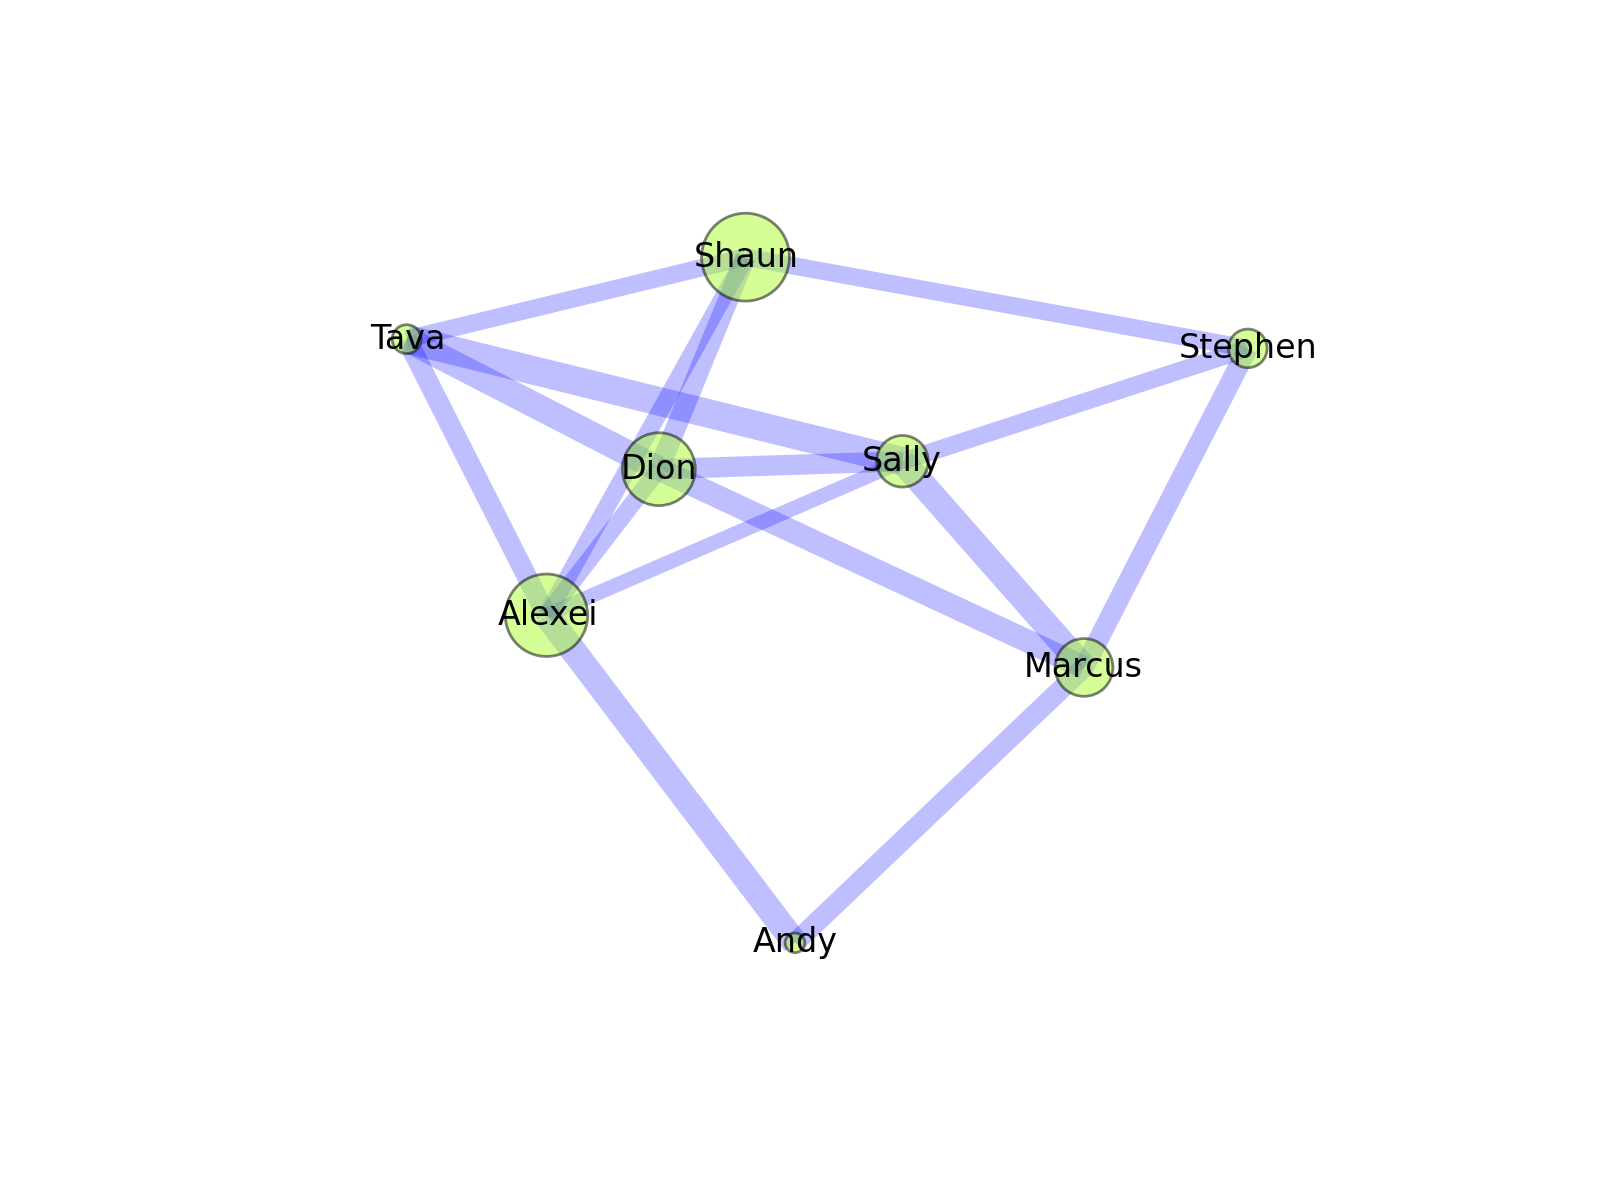
\includegraphics[width=.85\textwidth]{givers_random_network_example}
\caption{\label{fig:givers_random_network_example} 
A bunch of agents in a network, each with random behavioural parameters.  Node sizes indicate the utility at the end of the season, which was a couple of hundred gifts long. Links thicknesses indicate the total number of gifts exchanged (there's no indication here of which way they travelled though).  }\end{figure}

\begin{figure}[b]
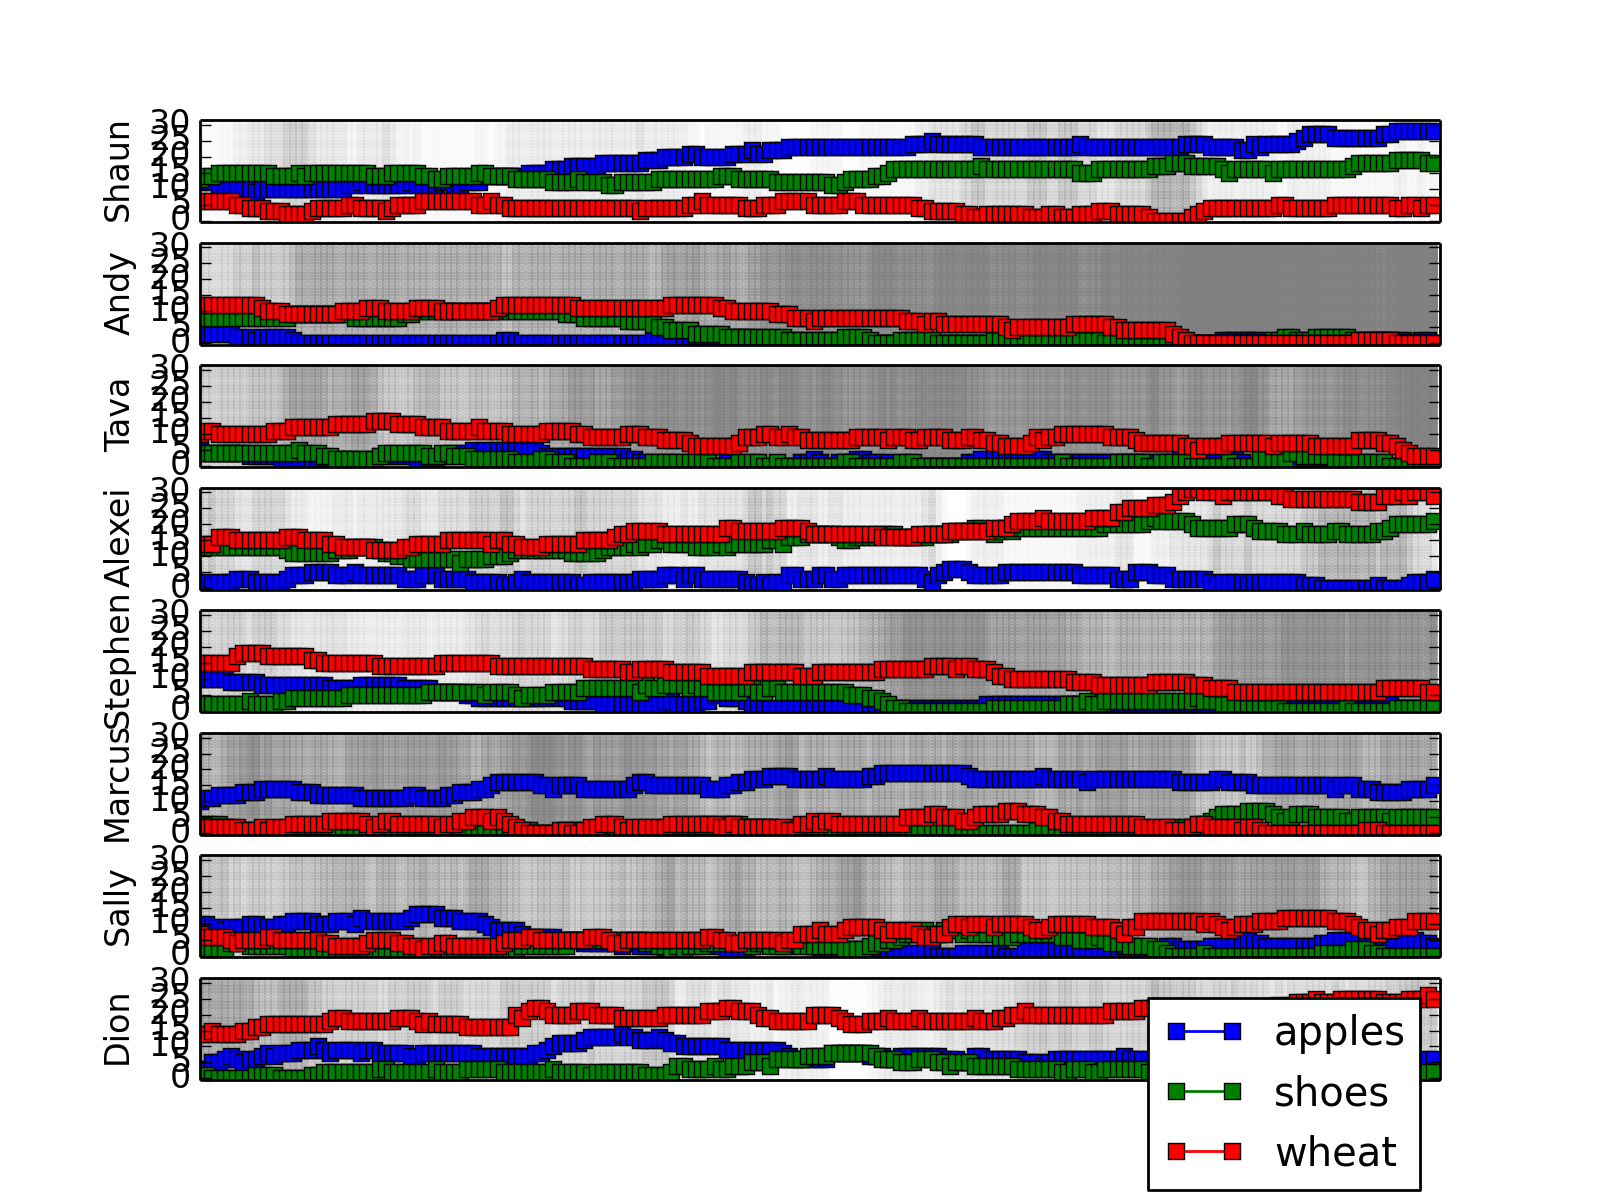
\includegraphics[width=\textwidth]{givers_random_network_example_seq}
\caption{\label{fig:givers_random_network_seq} 
The timecourse of commodity transfers leading to Figure \ref{fig:givers_random_network_example}. The gray background indicates the utility of the agent at that moment (with lighter background indicating higher utility). }\end{figure}


\section{conditional gifting can take over, I think}

See Figures \ref{fig:allTFT_good_memory_result}  and \ref{fig:allTFT_good_memory_seq} .

\begin{figure}[b]
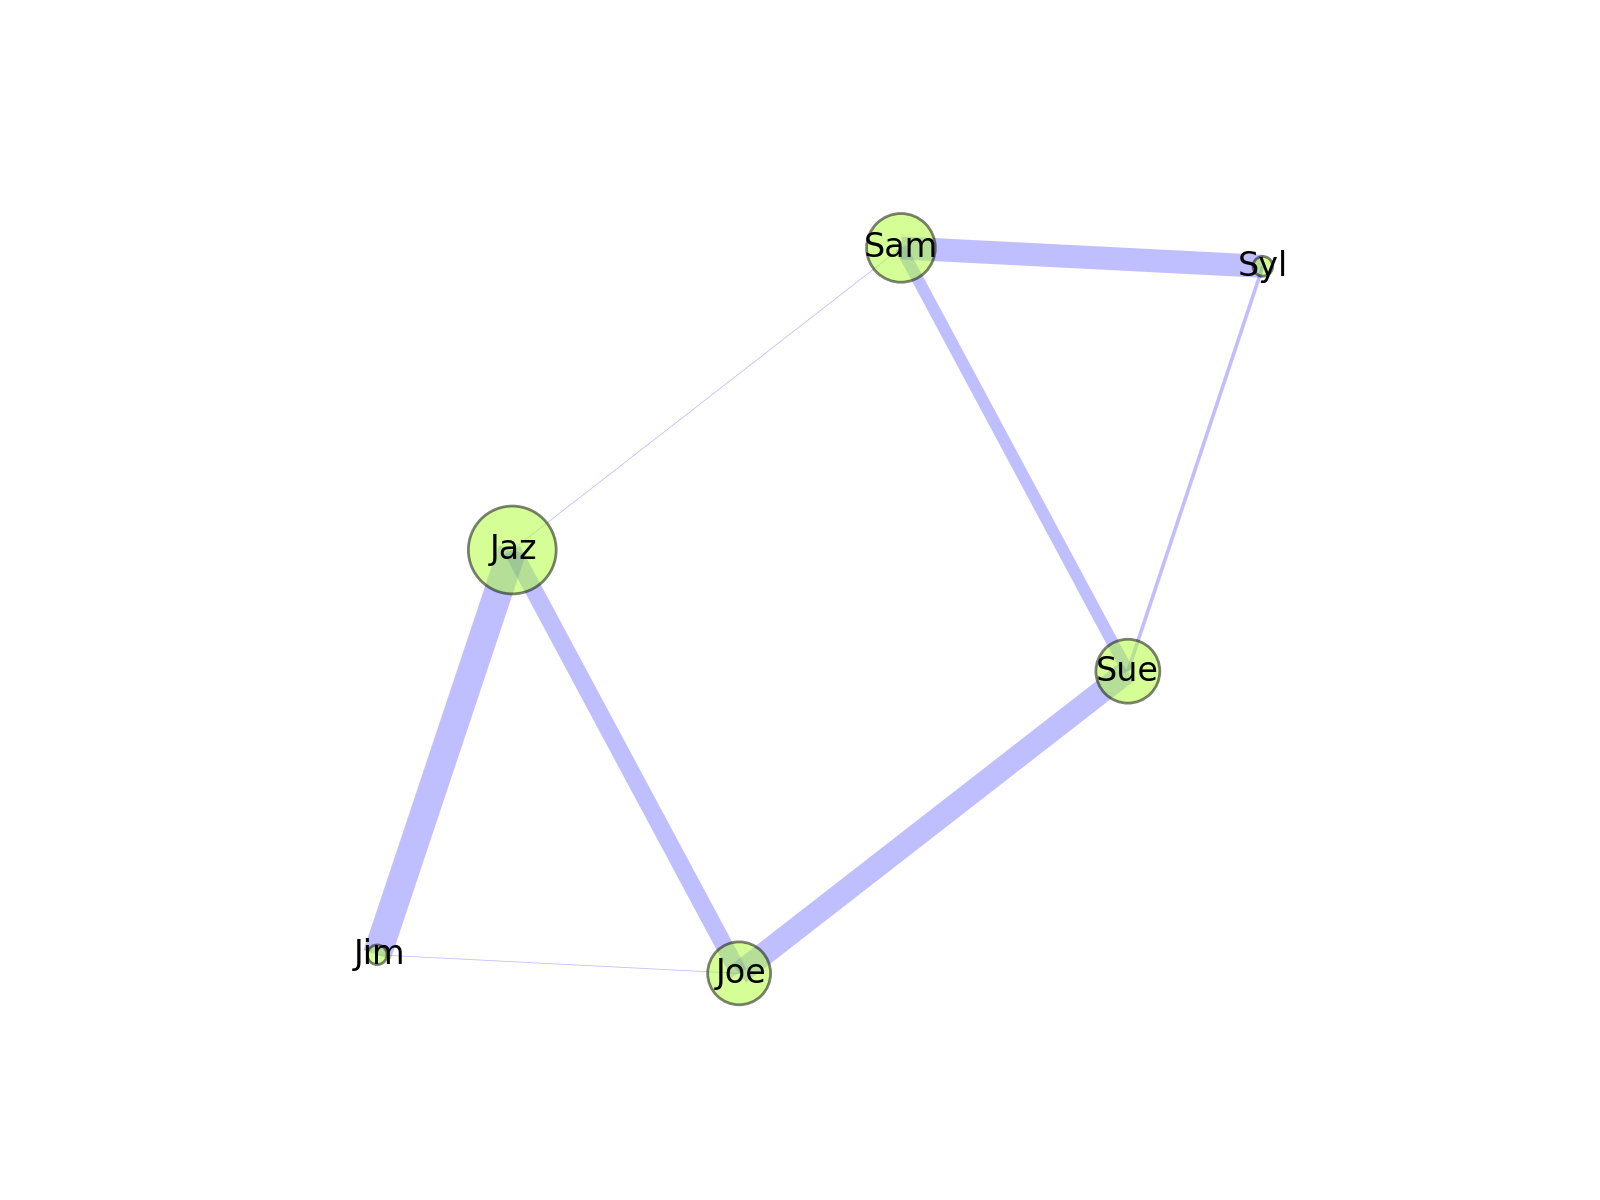
\includegraphics[width=.85\textwidth]{allTFT_good_memory_result}
\caption{\label{fig:allTFT_good_memory_result} 
Six agents, all playing a form of ``Tit for tat'', $w=(-1,5,10)$. There were 3 commodities, and each agent started off with just one of them in abundance and none of the others. Clearly a sub-network of reciprocating gifters has established, and the guys at the ``leaves'' (ends) are missing out on utility. }
\end{figure}

\begin{figure}[b]
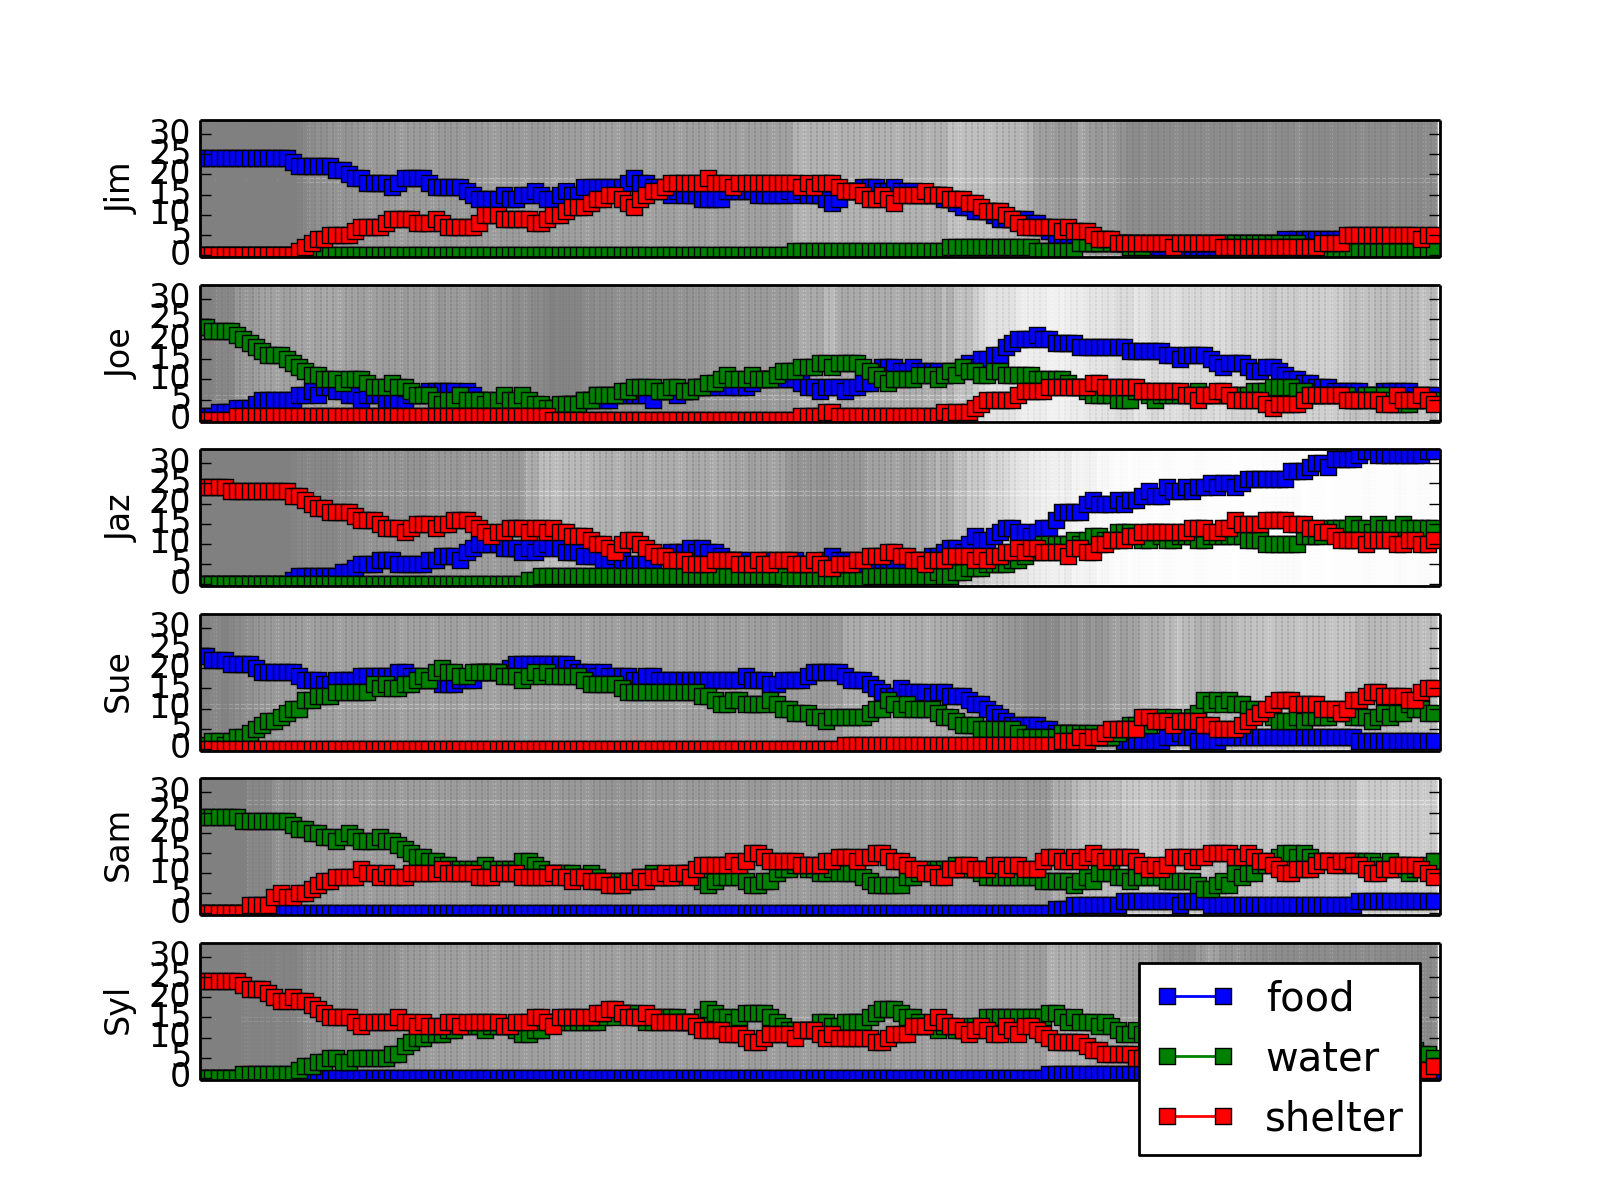
\includegraphics[width=\textwidth]{allTFT_good_memory_seq}
\caption{\label{fig:allTFT_good_memory_seq} 
The run leading to Figure \ref{fig:allTFT_good_memory_result} 
You can see that things got ugly for Jim at the end there.}
\end{figure}


Then it's interesting to split the network into some TFT players up against some
default guys who just don't (shed any gifts).

See Figures \ref{fig:twotribes_good_memory_result}  and \ref{fig:twotribes_good_memory_seq} .

\begin{figure}[b]
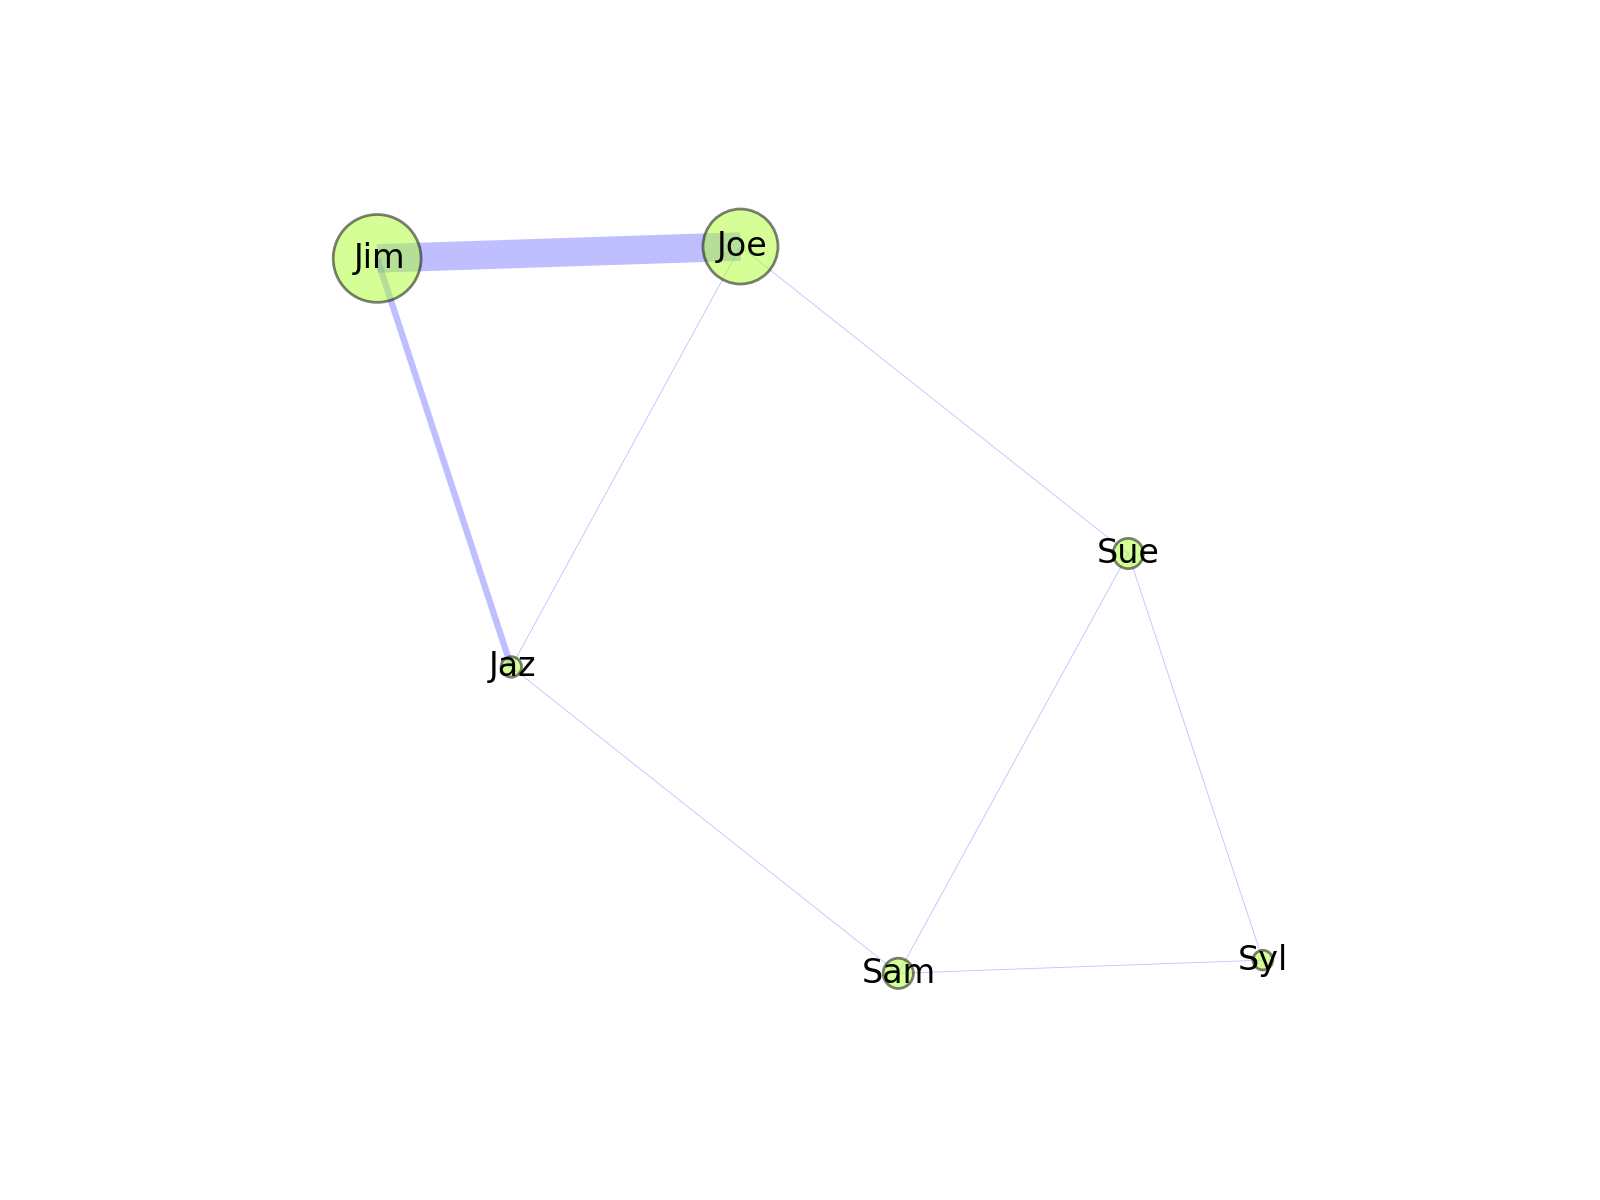
\includegraphics[width=.85\textwidth]{twotribes_good_memory_result}
\caption{\label{fig:twotribes_good_memory_result} 
The 3 amigos Jim, Joe and Jaz play ``Tit for tat'', $w=(-1,5,10)$, but the other three avoid giving anything away (ie. they only ever {\it receive} gifts).  {\bf Some of the TFT players come out on top (but some never get going). We might expect reciprocated gifting to spread, overall? }}
\end{figure}

\begin{figure}[b]
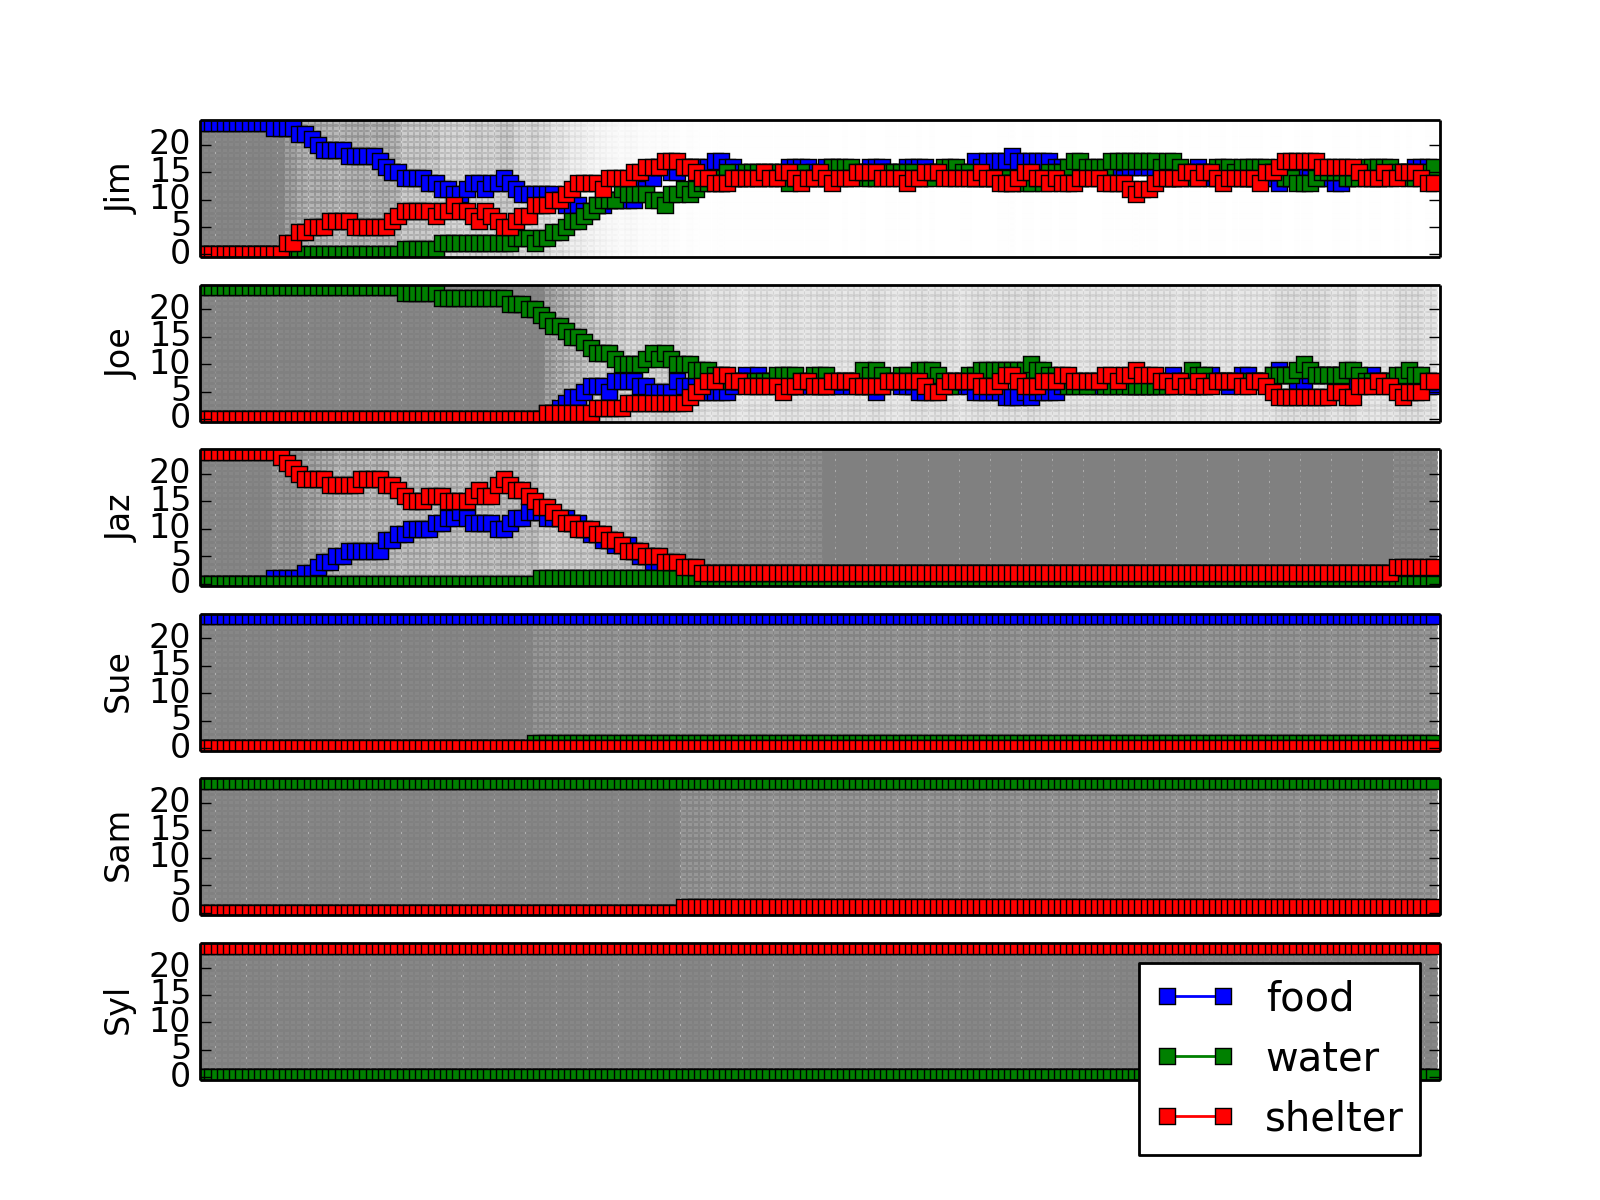
\includegraphics[width=\textwidth]{twotribes_good_memory_seq}
\caption{\label{fig:twotribes_good_memory_seq} 
The run leading to Figure \ref{fig:twotribes_good_memory_seq}. }
\end{figure}

So, even a bunch of identical TFT-like players end up trading in a
network that is a sub-net of the actual graph of neighbours. This
seems interesting. What causes it?

It seems to be a run-away effect of the tendency they have to
cooperate more with those they've cooperated with in the past,
essentially. They have perfect memory (ie. perfect accounting, at
least given the limitations imposed by the fact that they can only use
their own utilities in the current incarnation).

\section{what happens with shorter memories}

Perhaps limiting their memory will encourage them to ``share it
around'' more, although a good memory is perhaps the only thing that
allows them to defend themselves from the inveterate defectors as
well.

See Figures \ref{fig:allTFT_little_memory_result}  and \ref{fig:allTFT_little_memory_seq} .

\begin{figure}[b]
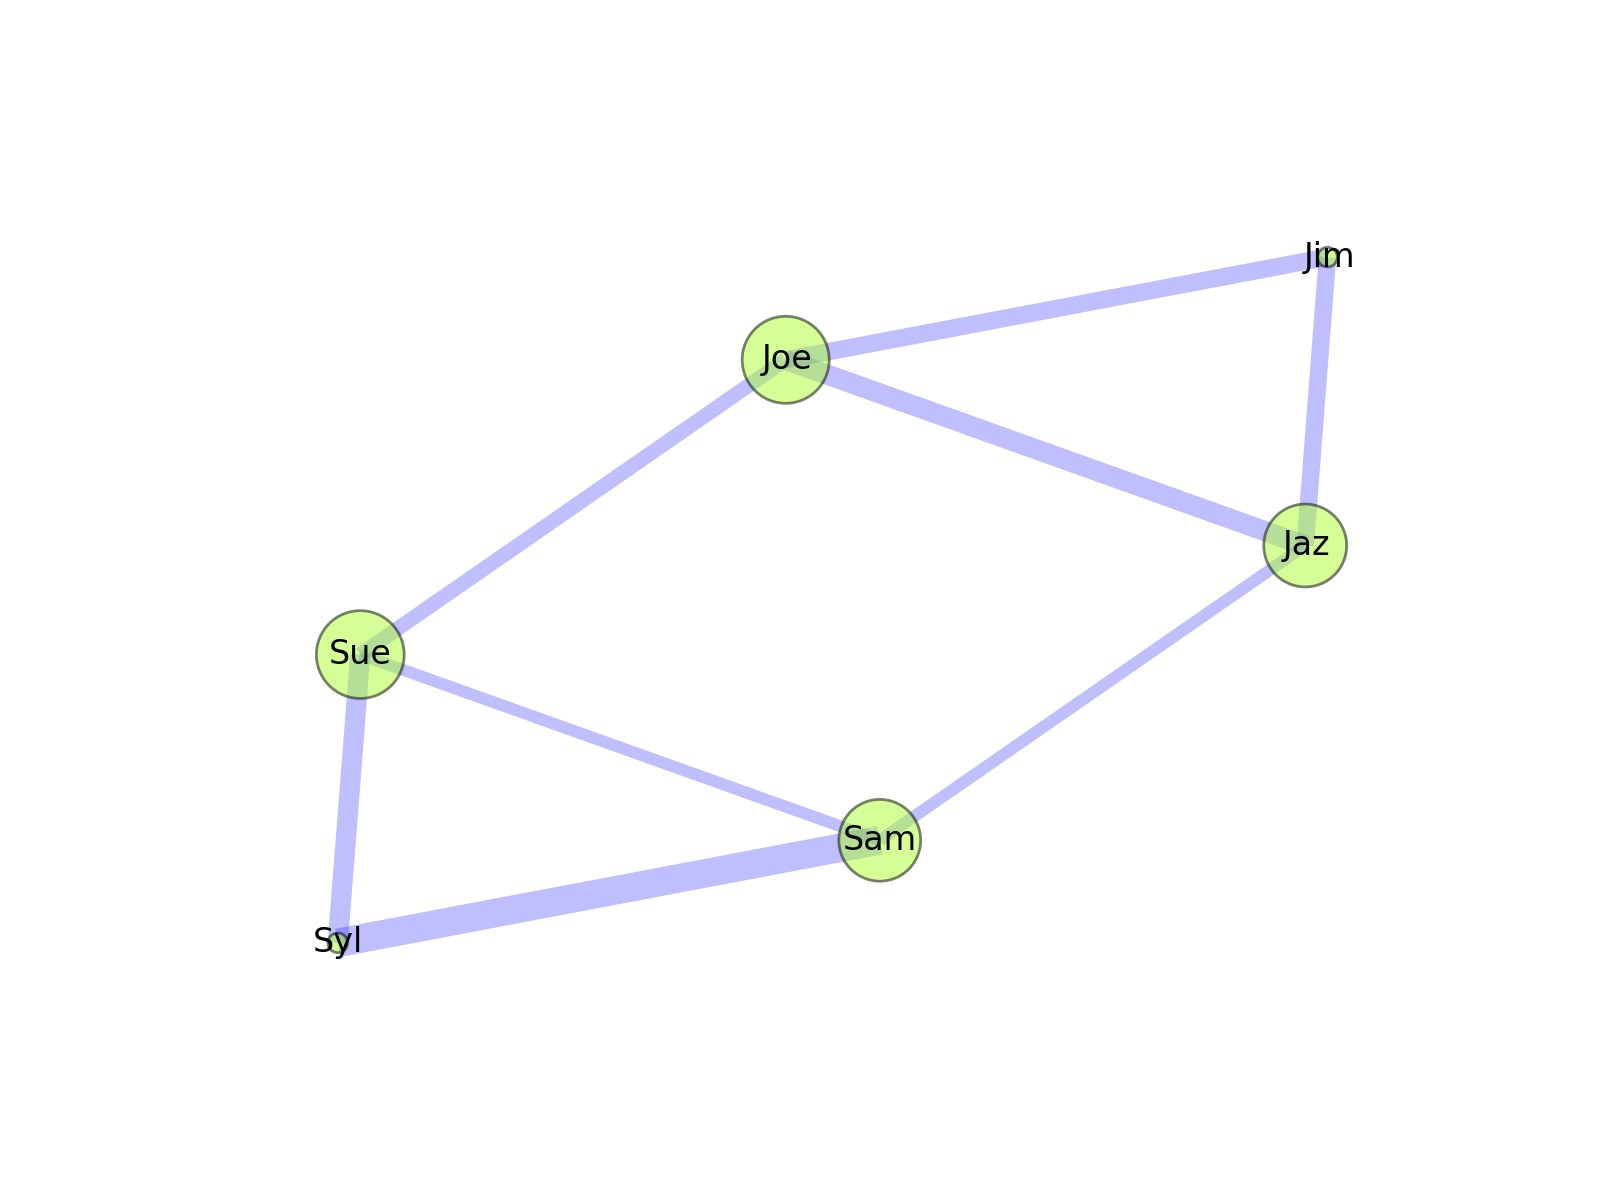
\includegraphics[width=.85\textwidth]{allTFT_little_memory_result}
\caption{\label{fig:allTFT_little_memory_result} 
First we try 6 agents, all playing a form of ``Tit for tat'' as before. But this time agents are slowly forgetting the ``debt'' they feel.  {\bf Huh?}}
\end{figure}

\begin{figure}[b]
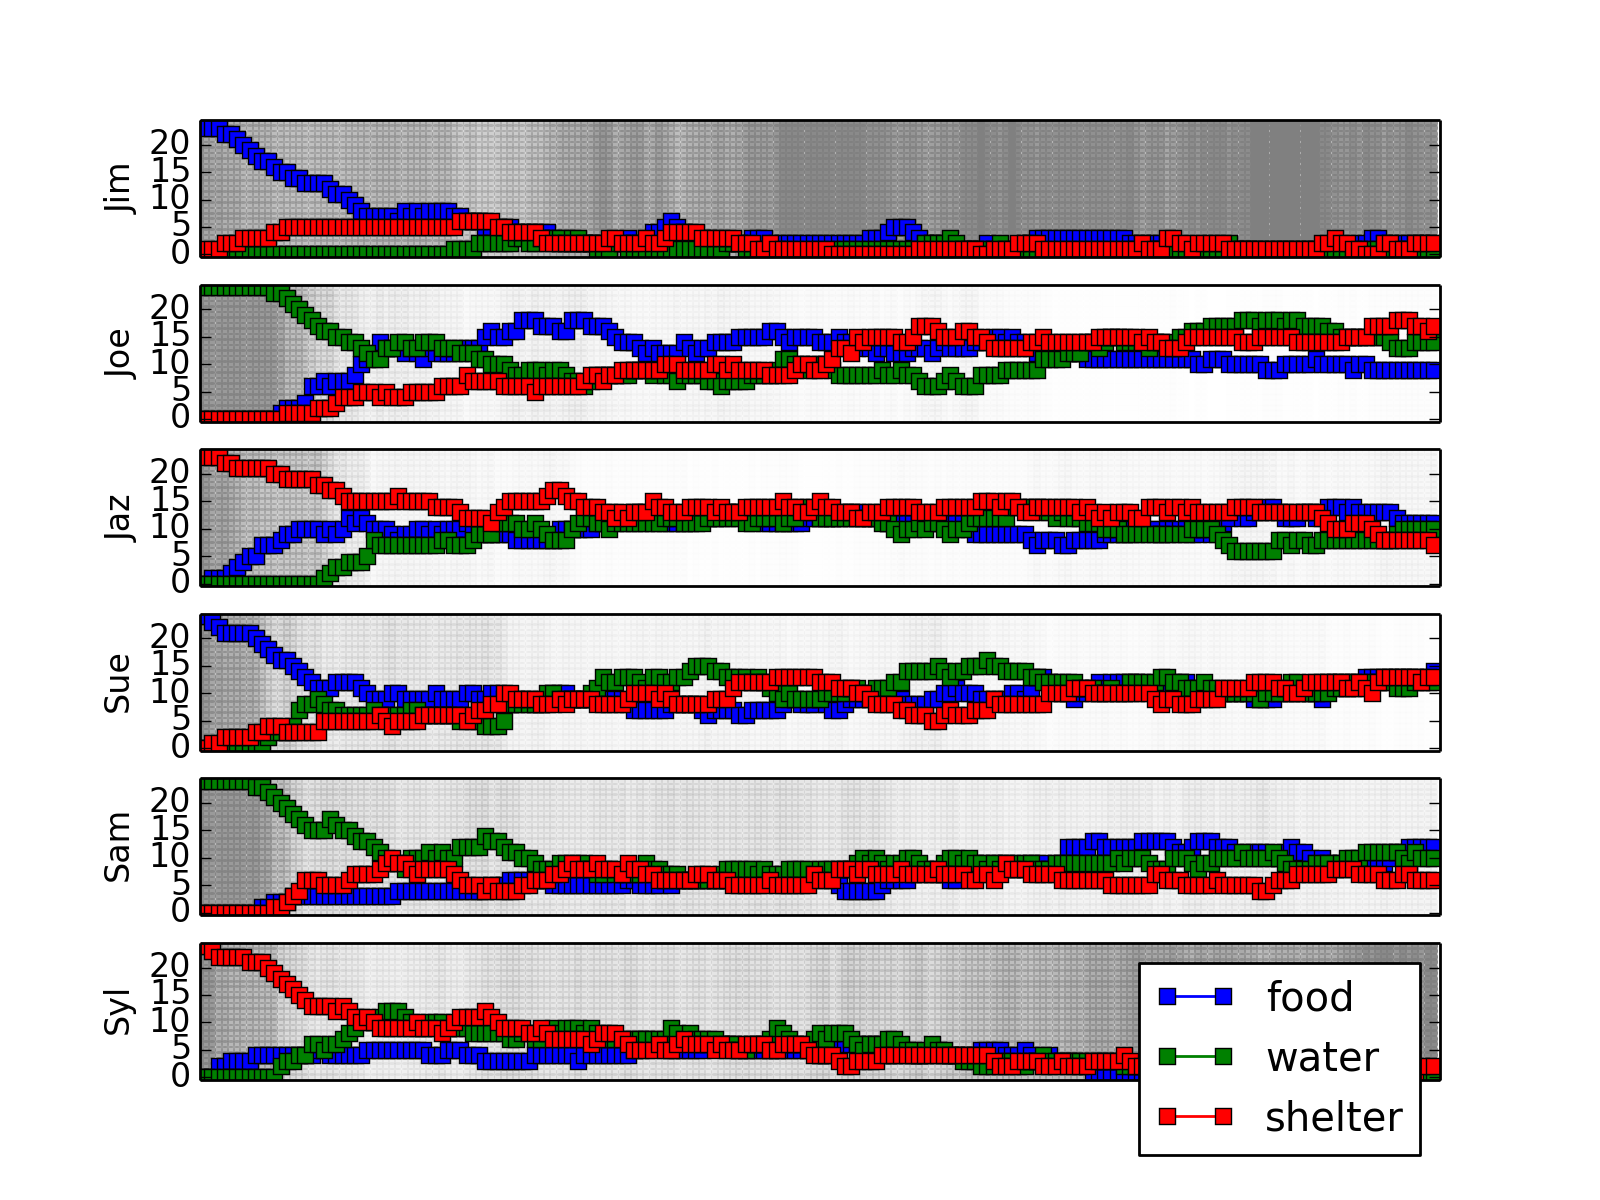
\includegraphics[width=\textwidth]{allTFT_little_memory_seq}
\caption{\label{fig:allTFT_little_memory_seq} 
The run leading to Figure \ref{fig:allTFT_little_memory_result} }
\end{figure}

\pagebreak

\begin{figure}[b]
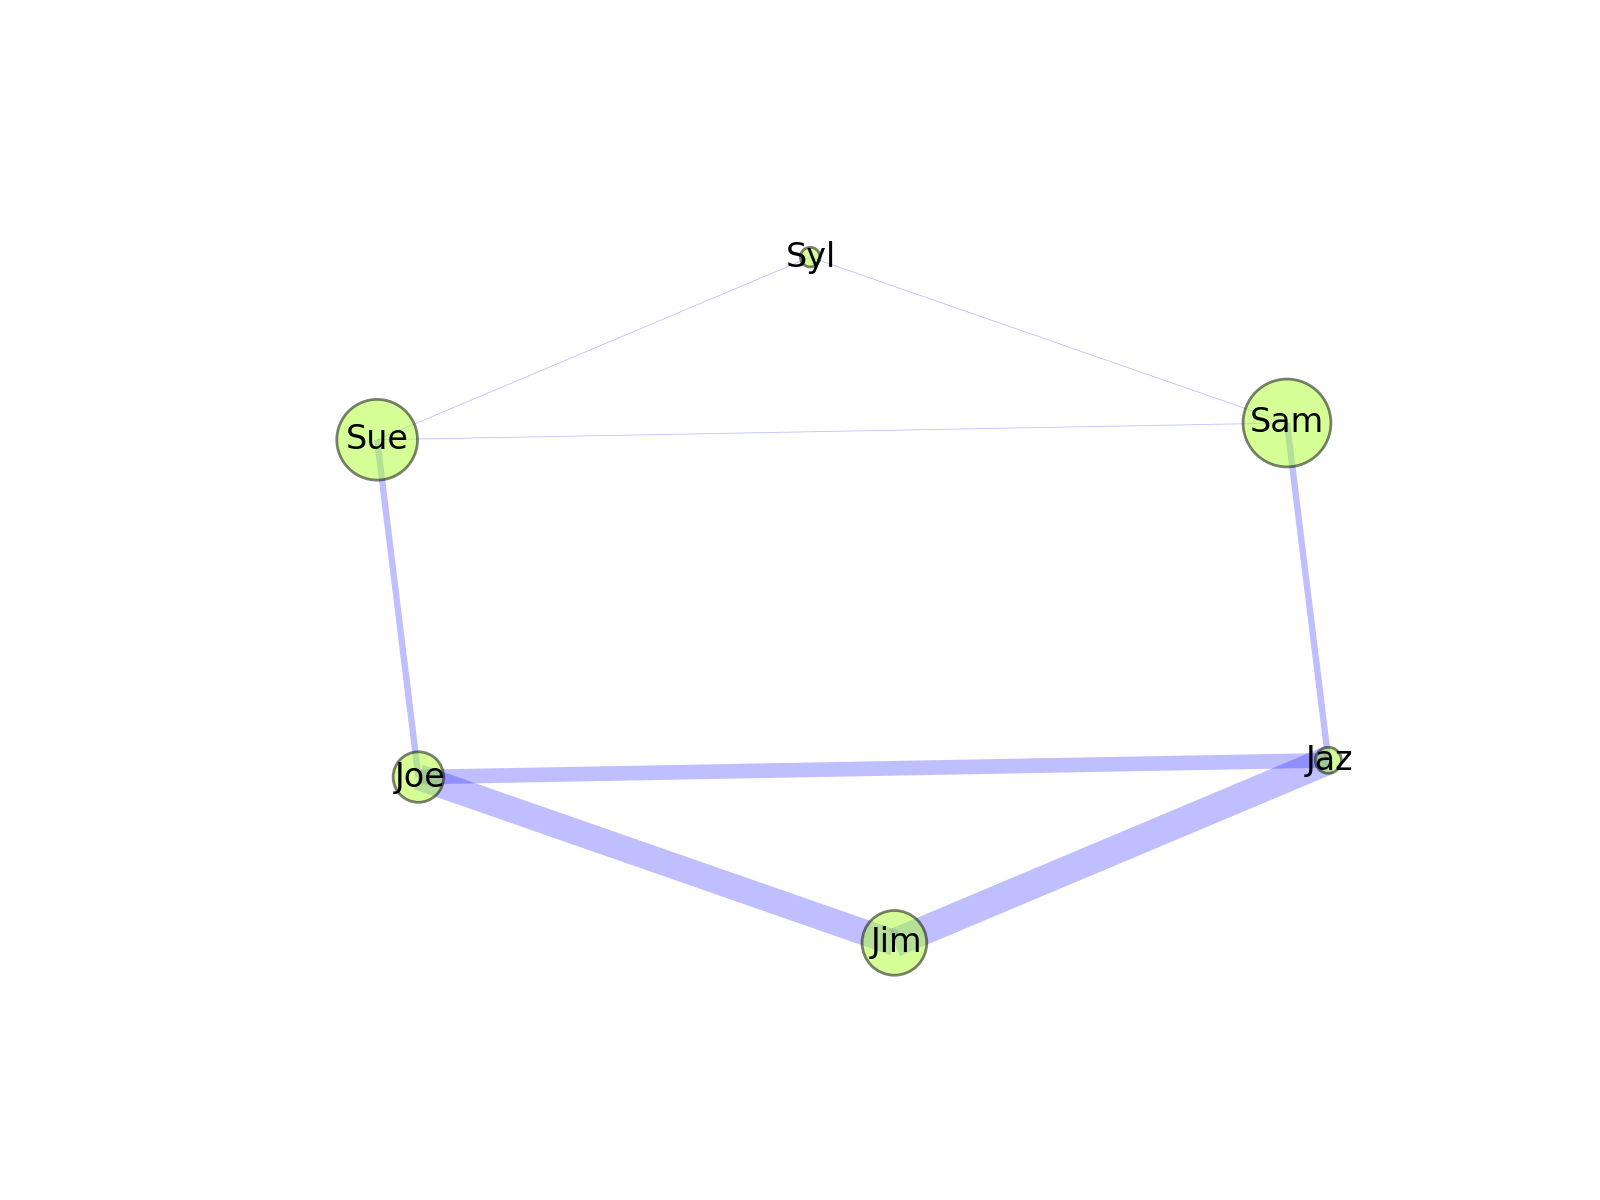
\includegraphics[width=.85\textwidth]{twotribes_little_memory_result}
\caption{\label{fig:twotribes_little_memory_result} 
The 3 amigos Jim, Joe and Jaz play ``Tit for tat'', $w=(-1,5,10)$, but the other three avoid giving anything away. {\bf The amigos all trade nicely with each other BUT Sue and Sam clean them up! Hilarious.} Presumably they keep forgetting that Sue and Sam are ripping them off.}
\end{figure}

\begin{figure}[b]
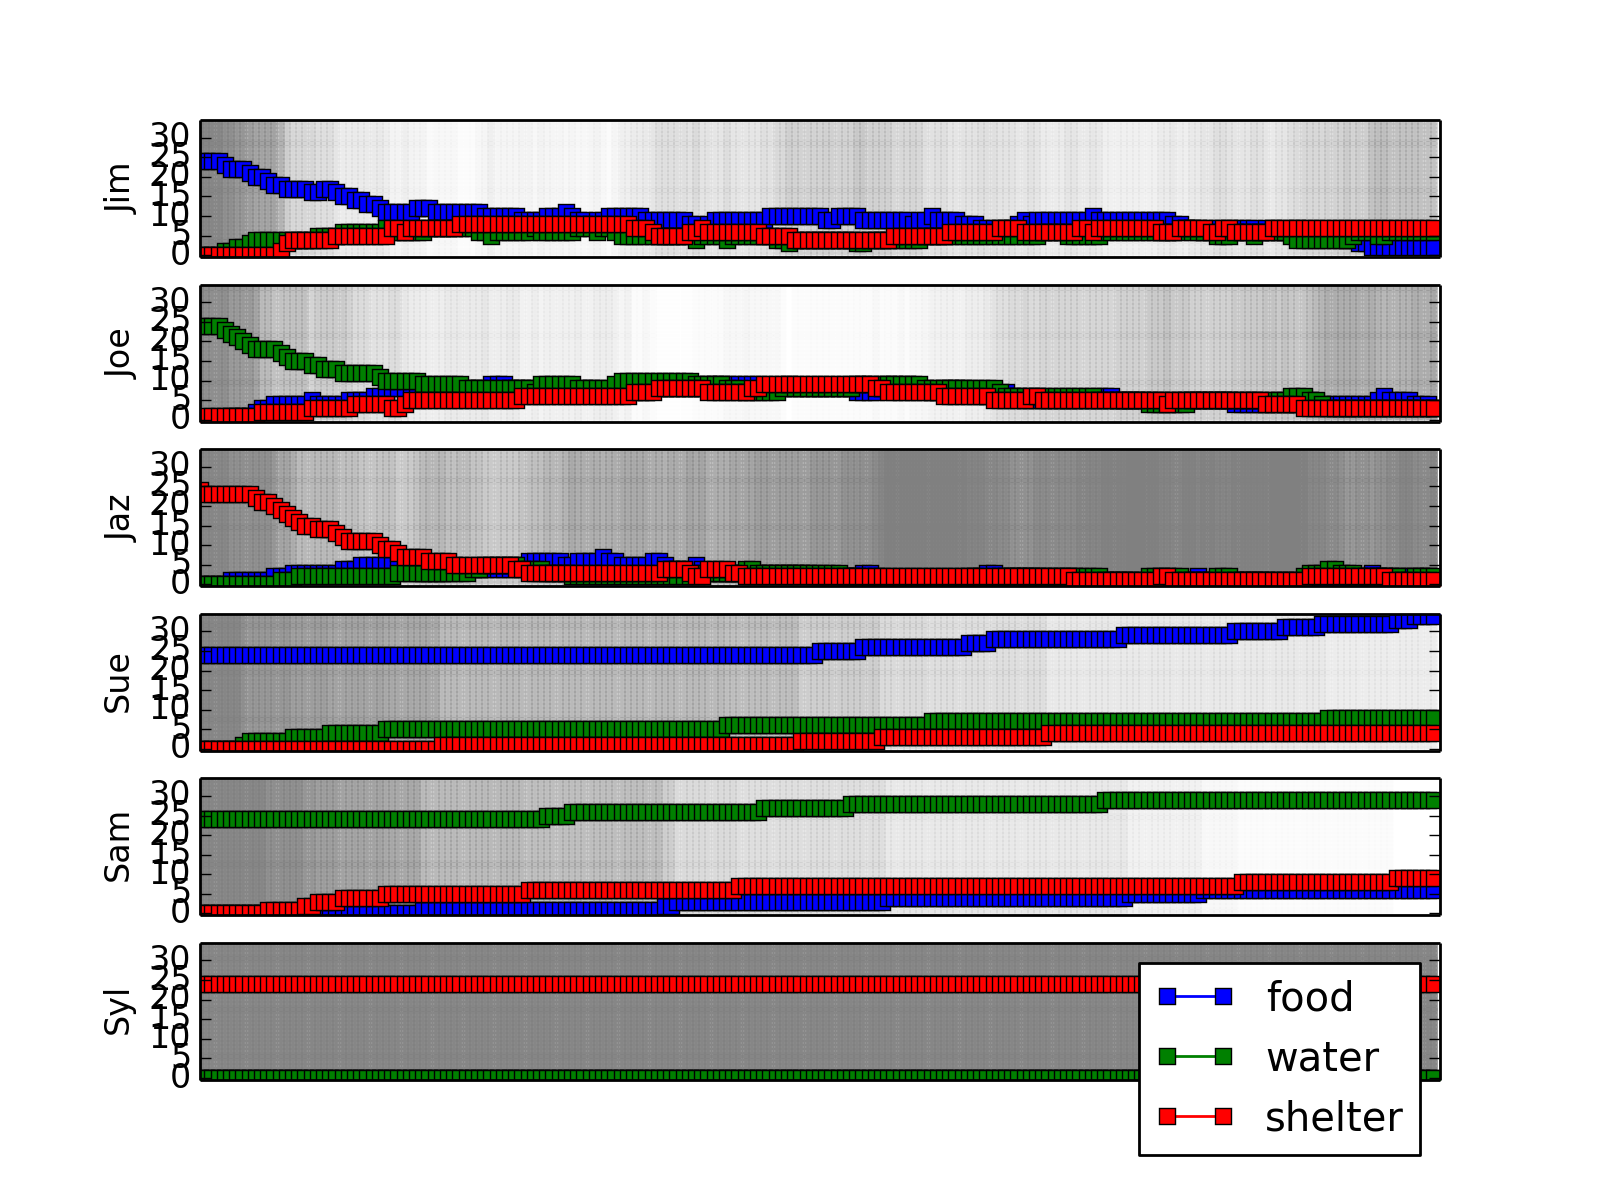
\includegraphics[width=\textwidth]{twotribes_little_memory_seq}
\caption{\label{fig:twotribes_little_memory_seq} 
The run leading to Figure \ref{fig:twotribes_little_memory_result} 
Joe and Jaz keep forgetting that Sue and Sam are ripping them off. Sheesh.}
\end{figure}

\section{Where to}

\begin{itemize}
\item it really sucks that I have this simple decision rule that looks like a friggn neuron and yet can't derive the infinite-time equilibrium distribution of commodities, even in the case of a ``network'' consisting of just two agents.
It hurts me that this is ``just a simulation''.
But is there a simpler formulation that's barter-capable?

\item obviously, want to ``evolve'' strategies (the weights), not prescribe them. Eg. start off all random, then every season every agent compares its own utility (average, final, whatever) to its neighbours, and simply adopts the weights of the best of those. We should see immediate collapse to nasty defection, and (perhaps much later...) eventual generation of TFTs that successfully invade the network. And THEN

\item I reckon agents should form better partnerships, and thrive, when they also take into account the utility of their gift {\it to the receiver} not just themselves. That's just another weight (assuming honest signalling is possible at any rate). Creatures able to do that should wipe out the first wave of cooperators. And THEN

\item We're inching towards the kind of scenario in which it's sensible to talk about the emergence of money. Maybe it comes in as a way to avoid the awkwardness caused by the (inevitable and considerable) differences between self-evaluated nett debts and other-evaluated nett debts?! Just a thought.
\end{itemize}

\end{document}

